\documentclass{article}
\usepackage[utf8]{inputenc}
\usepackage{hyperref}
\usepackage[letterpaper, portrait, margin=1in]{geometry}
\usepackage{enumitem}
\usepackage{amsmath}
\usepackage{booktabs}
\usepackage{graphicx}

\usepackage{hyperref}
\hypersetup{
colorlinks=true,
    linkcolor=black,
    filecolor=black,      
    urlcolor=blue,
    citecolor=black,
}
\usepackage{natbib}

\usepackage{titlesec}
  
\title{ECON 7103 Homework 2}
\author{Yifan Liu (yliu3494)}
\date{Spring 2023}
  
\begin{document}
  
\maketitle




\section{Python}
The randomization of grouping worked. There is no significant difference in square feet of the home and the outdoor average temperature between the treatment and control groups.

\begin{table}[hbt!]
    \centering
    \begin{tabular}{llll}
\toprule
{} &          Mean &           Mean  &           P-value  \\
{} &        (s.d.) &          (s.d.) &          of t-test \\
{} & control group & treatment group & between two groups \\
\midrule
electricity &       1181.33 &         1086.75 &         0.00069222 \\
            &      (454.31) &        (423.96) &                    \\
sqft        &       1633.05 &         1657.55 &            0.57163 \\
            &      (682.90) &        (686.27) &                    \\
temp        &         79.89 &           79.89 &           0.987135 \\
            &        (2.16) &          (1.97) &                    \\
\bottomrule
\end{tabular}

    \caption{Sample mean, sample standard deviations, and p-values for the two-way t-test between treatment and control group means}
    \label{tab:table_Q1}
\end{table}


\begin{figure}[hbt!]
    \centering
    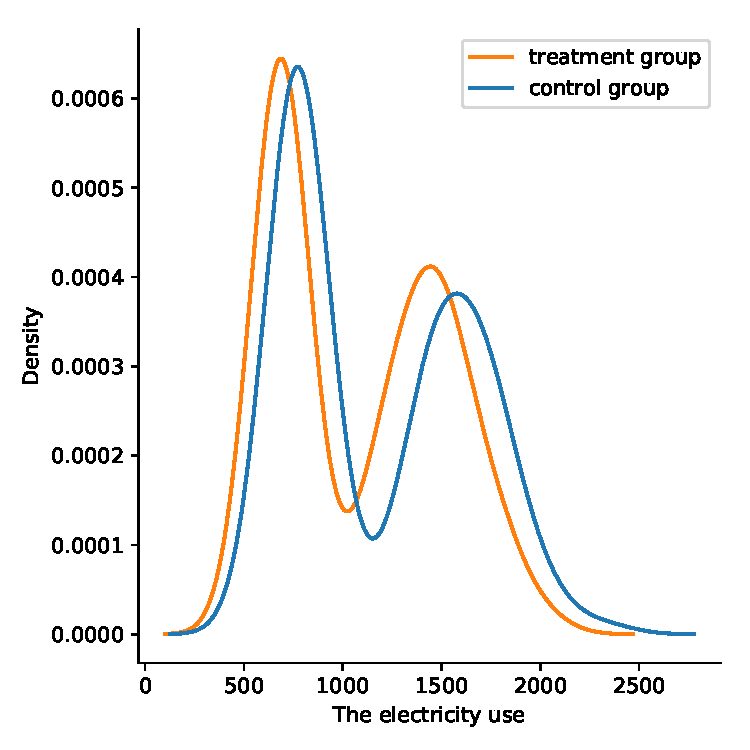
\includegraphics[scale = 0.7]{hist_Q2.pdf}
    \caption{Kernel density plot of the electricity use for treated group and control group}
    \label{fig:hist_Q2}
\end{figure}

Figure 1 provides graphical evidence that the retrofits worked. The energy consumption distribution of the treatment group is on the slightly left side of the control group. In other words, receiving the energy-efficiency retrofit program makes households consume less electricity. 

\hspace{1cm}

Below Table 2 presents the coefficients of three OLS estimation techniques.

\begin{table}[hbt!]
    \centering
    \begin{tabular}{llll}
\toprule
{} &          Mean &           Mean  &           P-value  \\
{} &        (s.d.) &          (s.d.) &          of t-test \\
{} & control group & treatment group & between two groups \\
\midrule
electricity &       1181.33 &         1086.75 &         0.00069222 \\
            &      (454.31) &        (423.96) &                    \\
sqft        &       1633.05 &         1657.55 &            0.57163 \\
            &      (682.90) &        (686.27) &                    \\
temp        &         79.89 &           79.89 &           0.987135 \\
            &        (2.16) &          (1.97) &                    \\
\bottomrule
\end{tabular}

    \caption{Coefficients of three OLS estimation techniques}
    \label{tab: table_Q3}
\end{table}


\section{Stata}

Table 3 below displays each variable's sample, sample standard deviation, and p-values for the two-way t-test between treatment and control groups.

\begin{table}[hbt!]
    \centering
    {
\def\sym#1{\ifmmode^{#1}\else\(^{#1}\)\fi}
\begin{tabular}{l*{3}{c}}
\hline\hline
                    &\multicolumn{1}{c}{(1)}&\multicolumn{1}{c}{(2)}&\multicolumn{1}{c}{(3)}\\
                    &\multicolumn{1}{c}{}&\multicolumn{1}{c}{}&\multicolumn{1}{c}{}\\
                    &Mean/Std. Dev.&Mean/Std. Dev.&Mean/Std. Dev.\\
\hline
electricity         &     1181.33&     1086.75&            \\
                    &    (454.31)&    (423.96)&            \\
sqft                &     1633.05&     1657.55&            \\
                    &    (682.90)&    (686.27)&            \\
temp                &       79.89&       79.89&            \\
                    &      (2.16)&      (1.97)&            \\
\hline
Observations        &         501&         499&        1000\\
\hline\hline
\end{tabular}
}

    \caption{Sample mean, sample standard deviations, and p-values for the two-way t-test between treatment and control group means}
    \label{tab:stata_Q1}
\end{table}

Figure 2 below is a two-way scatter plot with electricity consumption on the y-axis and square feet on the x-axis. We can have a general idea that the electricity consumption per household is positively related to the size of the home.

\begin{figure}[hbt!]
    \centering
    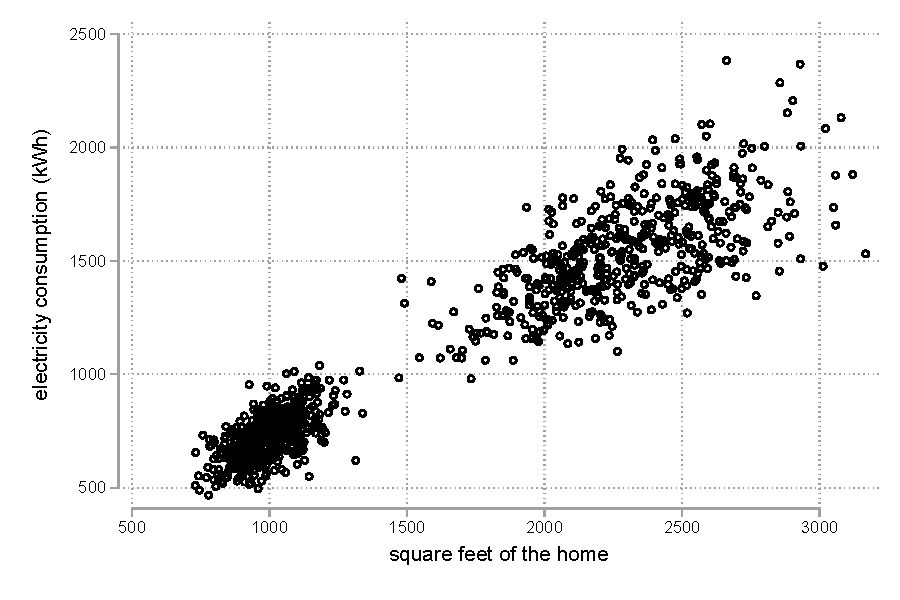
\includegraphics[scale = 0.7]{stata_Q2.pdf}
    \caption{Two-way scatterplot of electricity consumption against square fee of the home}
    \label{fig:stata_Q2}
\end{figure}

\hspace{1cm}

Table 4 shows the regression result with heteroskedasticity-robust standard errors.

\begin{table}[hbt!]
    \centering
    \begin{tabular}{lc} \hline
 & (1) \\
VARIABLES & Ordinary least squares \\ \hline
 &  \\
sqft & 0.62** \\
 & (0.01) \\
retrofit & -109.67** \\
 & (7.94) \\
temp & 3.26 \\
 & (1.93) \\
Constant & -83.60 \\
 & (154.69) \\
 &  \\
Observations & 1,000 \\
 R-squared & 0.92 \\ \hline
\multicolumn{2}{c}{ Robust standard errors in parentheses} \\
\multicolumn{2}{c}{ ** p$<$0.01, * p$<$0.05} \\
\end{tabular}

    \caption{Regreesion results}
    \label{tab:stata_Q3}
\end{table}


\end{document}